\subsubsection{Purpose}
The use car feature is the key feature of the whole system. For the sake of completeness, this requirement is described by detailing each of its sub-parts, as seen in Figure \ref{global_uc}.

The detailed sub-parts are described in the subsections immediately after this one, namely: section \ref{unlock_car_section}, section \ref{start_ride_section}, \ref{end_ride_section} and \ref{apply_charges_section}. As a consequence, the scenarios provided in this subsection are general and must be considered in conjunction with the more detailed one to have a full overview of the use-case.

Its purpose is that of allowing users to open, get on and drive the actual vehicle that they rented via the dedicated service. This feature requires the interaction of the user with both his/her mobile device and the on-board computer application.

The system must unlock a car upon the performance of the authentication method from the user that reserved it. The on-board computer application must keep track of every important detail of user rides, such as the current charges, the nearby free charging spots and the boundaries of the Safe Area, all while notifying correspondingly the driver.

The on-board computer application will detect the beginning and end of the ride, counting the charges accordingly. Also, the system will be able to detect whether the car is inside the Safe Area or not: if this is not the case, the user will be notified and the charges will keep increasing.

This feature triggers the notifications sent to the existing maintenance system, as it includes the detection of out-of-service vehicles.

\subsubsection{Scenario 1}
Vincent reserved a \emph{PowerEnJoy} car to reach a far destination within his city. He reaches the vehicle and unlocks the car with his smartphone's GPS. Once aboard, he performs the authentication procedure and turns the car on, then starts his ride. Arrived at his destination, Vincent pulls over and checks that he did not park outside the Safe Area: since he did not, he turns the engine on and gets off the car. The system locks the car and applies all charges, initiating the automatic payment process.

\subsubsection{Scenario 2}
Wanda decided to rent a shared car instead of taking the subway train home. She reserved one on \emph{PowerEnJoy} and is now walking towards it. She unlocks the car properly and gets on it; after proper authentication, she starts driving. Her house is a the opposite border of the Safe Area, so she drives for a long time before arriving to her destination. Once she stops the engine, the system recognizes that the battery level is below 20\%: it immediately proceeds to check the vicinity for charging stations. The system does not find any nearby so, after 5 minutes, it marks the car as "out-of-service", and Wanda is charged the correct amount of money for the ride.

\subsubsection{Use-case}
A general use-case analysis is provided in Table \ref{use_car_uc}. The subparts are detailed in the following subsections as specified in "Purpose" above. \\
A statechart of the possible states of a car is shown in Figure \ref{use_car_sc}.

\subsubsection{Functional Requirements}
The requirements listed below do not include the ones covered within the sub-parts mentioned above. To have a detailed overview of all the requirements related to the sub-functionalities, see the subsections mentioned in "Purpose".

\begin{enumerate}
\item The system must keep track of the position of all vehicles in use;
\item The system must mark as "out-of-service" every vehicle that broke down;
\item The system must mark as "out-of-service" every vehicle that ran out of battery charge;
\item The system must mark as "out-of-service" the vehicles that were parked with more than 80\% of the battery empty and is not plugged into a power grid;
\item The system must mark as "available" the vehicles that were parked with more than 20\% of the battery still full;
\item As soon as a vehicle is marked as "out-of-service", a notification is sent over to the maintenance system.
\item If more than 15 minutes pass between a car being unlocked and it being turned on, the system must mark the vehicle as "out-of-service" and prevent it from being used;
\end{enumerate}

\begin{table}[H]
\begin{center}
\begin{tabular}{p{0.3\textwidth} | p{0.7\textwidth}}
\hline
Actor & User\\
\hline
Goal & Goal 7\\
\hline
Input Condition & The user reserved a car and reaches its location.\\
\hline
Event Flow & 
\begin{enumerate}
\item The user unlocks the car (see detail in section \ref{unlock_car_section});
\item The user authenticates and ingnites the engine, starting his/her ride (see detail in section \ref{start_ride_section});
\item The user rides the rented car to his/her destination;
\item The user ends his/her ride (see detail in section \ref{end_ride_section});
\item The system applies all charges, including additional ones and eventual discounts (see detail in section \ref{apply_charges_section});
\end{enumerate} \\
\hline
Output Condition & After the end of the ride and a 5 minute period used to perform eventual additional checks, the user ends the use of the service.\\
\hline
Exception & If the ride ends and the battery is more than 80\% empty, the vehicle is marked as "out-of-order" instead of "available".

If the car is involved in an accident or breaks down, the ride ends and the vehicle is marked as "out-of order" immediately. The user is charged only up to the amount corresponding to the instant before the accident. Note that accidents include the eventuality of the car running out of battery charge during the ride.

If more than 15 minutes pass between a car being unlocked and it being turned on, the vehicle is marked as "out-of-service"; the maintenance team is in charge of checking the car situation.\\
\hline
\end{tabular}
\end{center}
\caption{Use car general use-case}
\label{use_car_uc}
\end{table}

\begin{figure}[H]
\begin{center}
		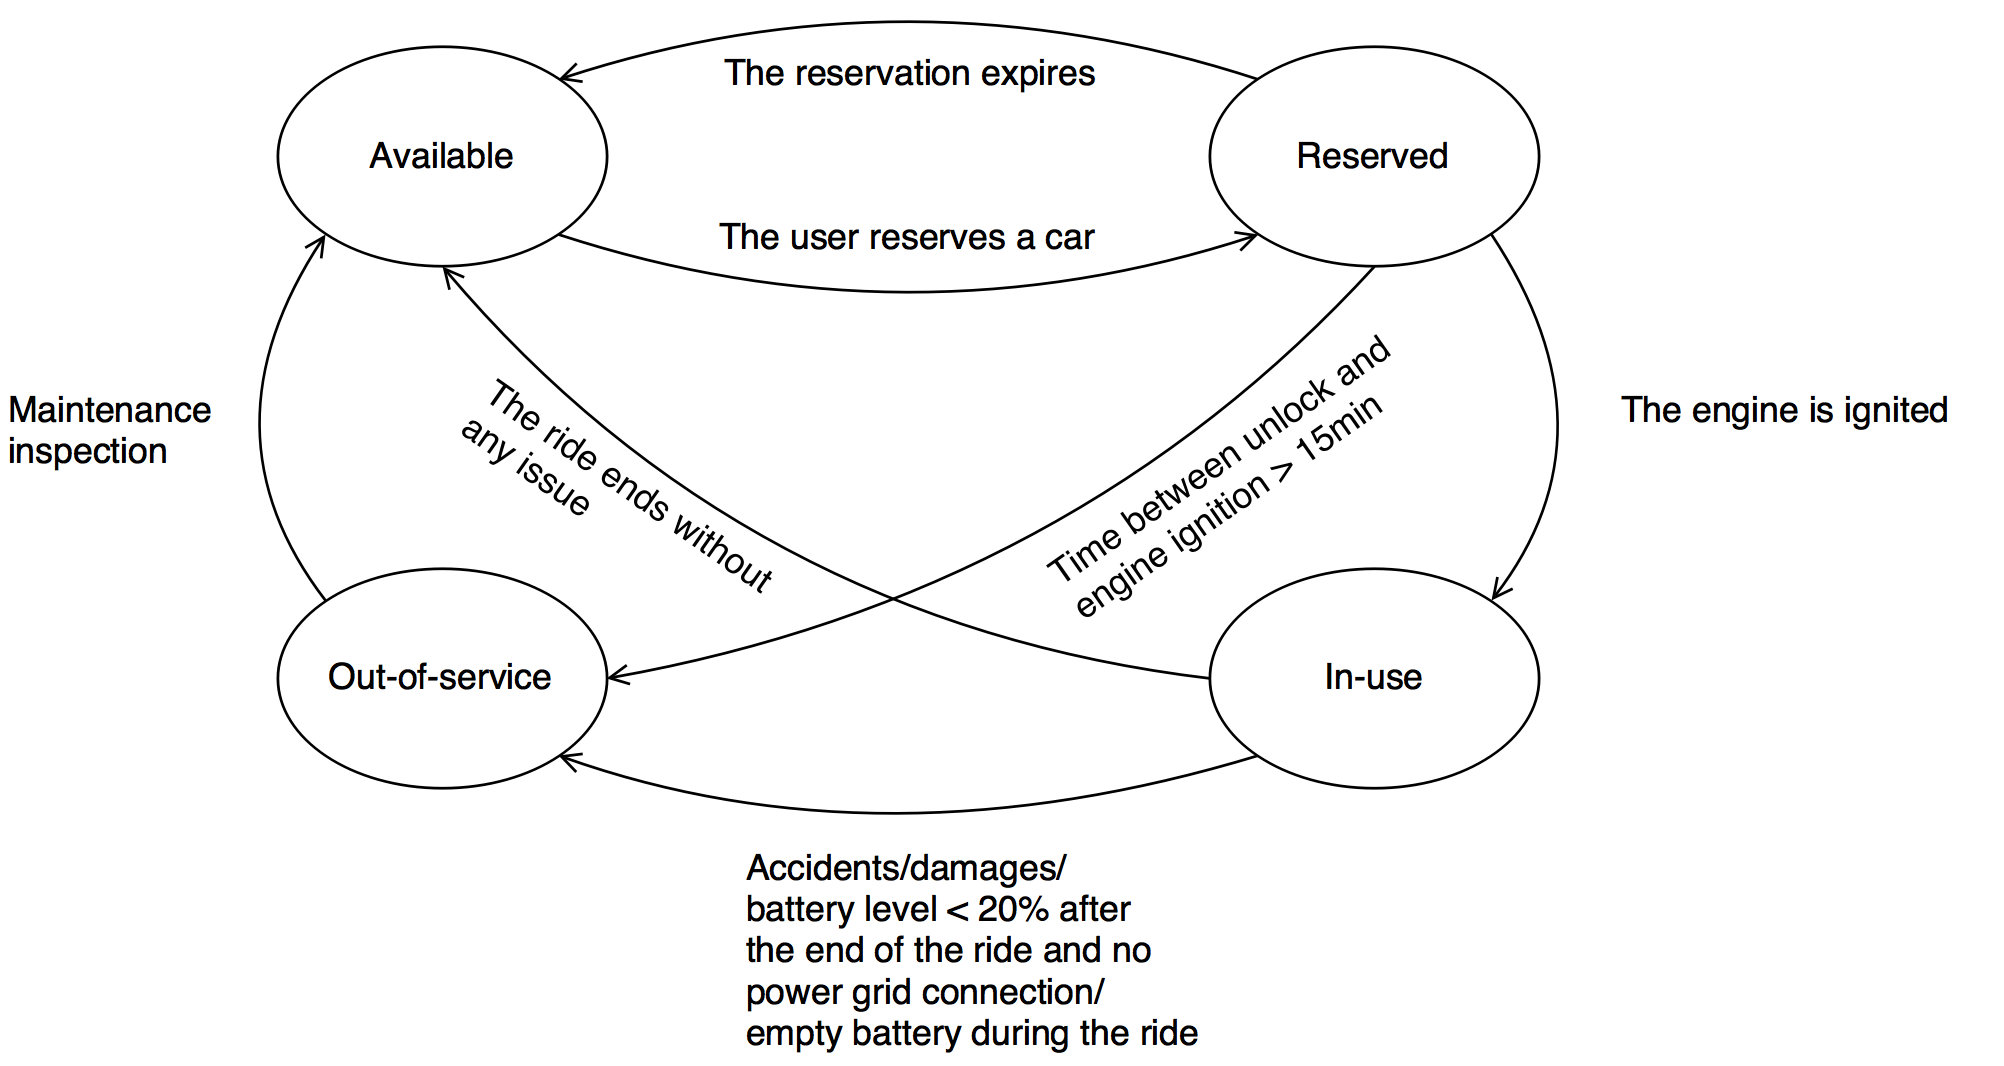
\includegraphics[width=\textwidth]{./specific_requirements/features/diagrams/use_car_sc.png}
		\caption{Statechart of the car usage.}
		\label{use_car_sc}
\end{center}
\end{figure}